\section{Senzor výšky hladiny}
\label{sec:perif-sensor-hladina}
    Voda v akváriu se průběžně odpařuje a je potřeba ji doplňovat. Účelem této periferie je průběžné monitorování hladiny akvária a upozornění uživatele na nutnost doplnění vody. Také může uživatele varovat v případě poškození nádrže a nežádoucího úniku vody do okolí. 

    \begin{figure}[h!]
        \centering
        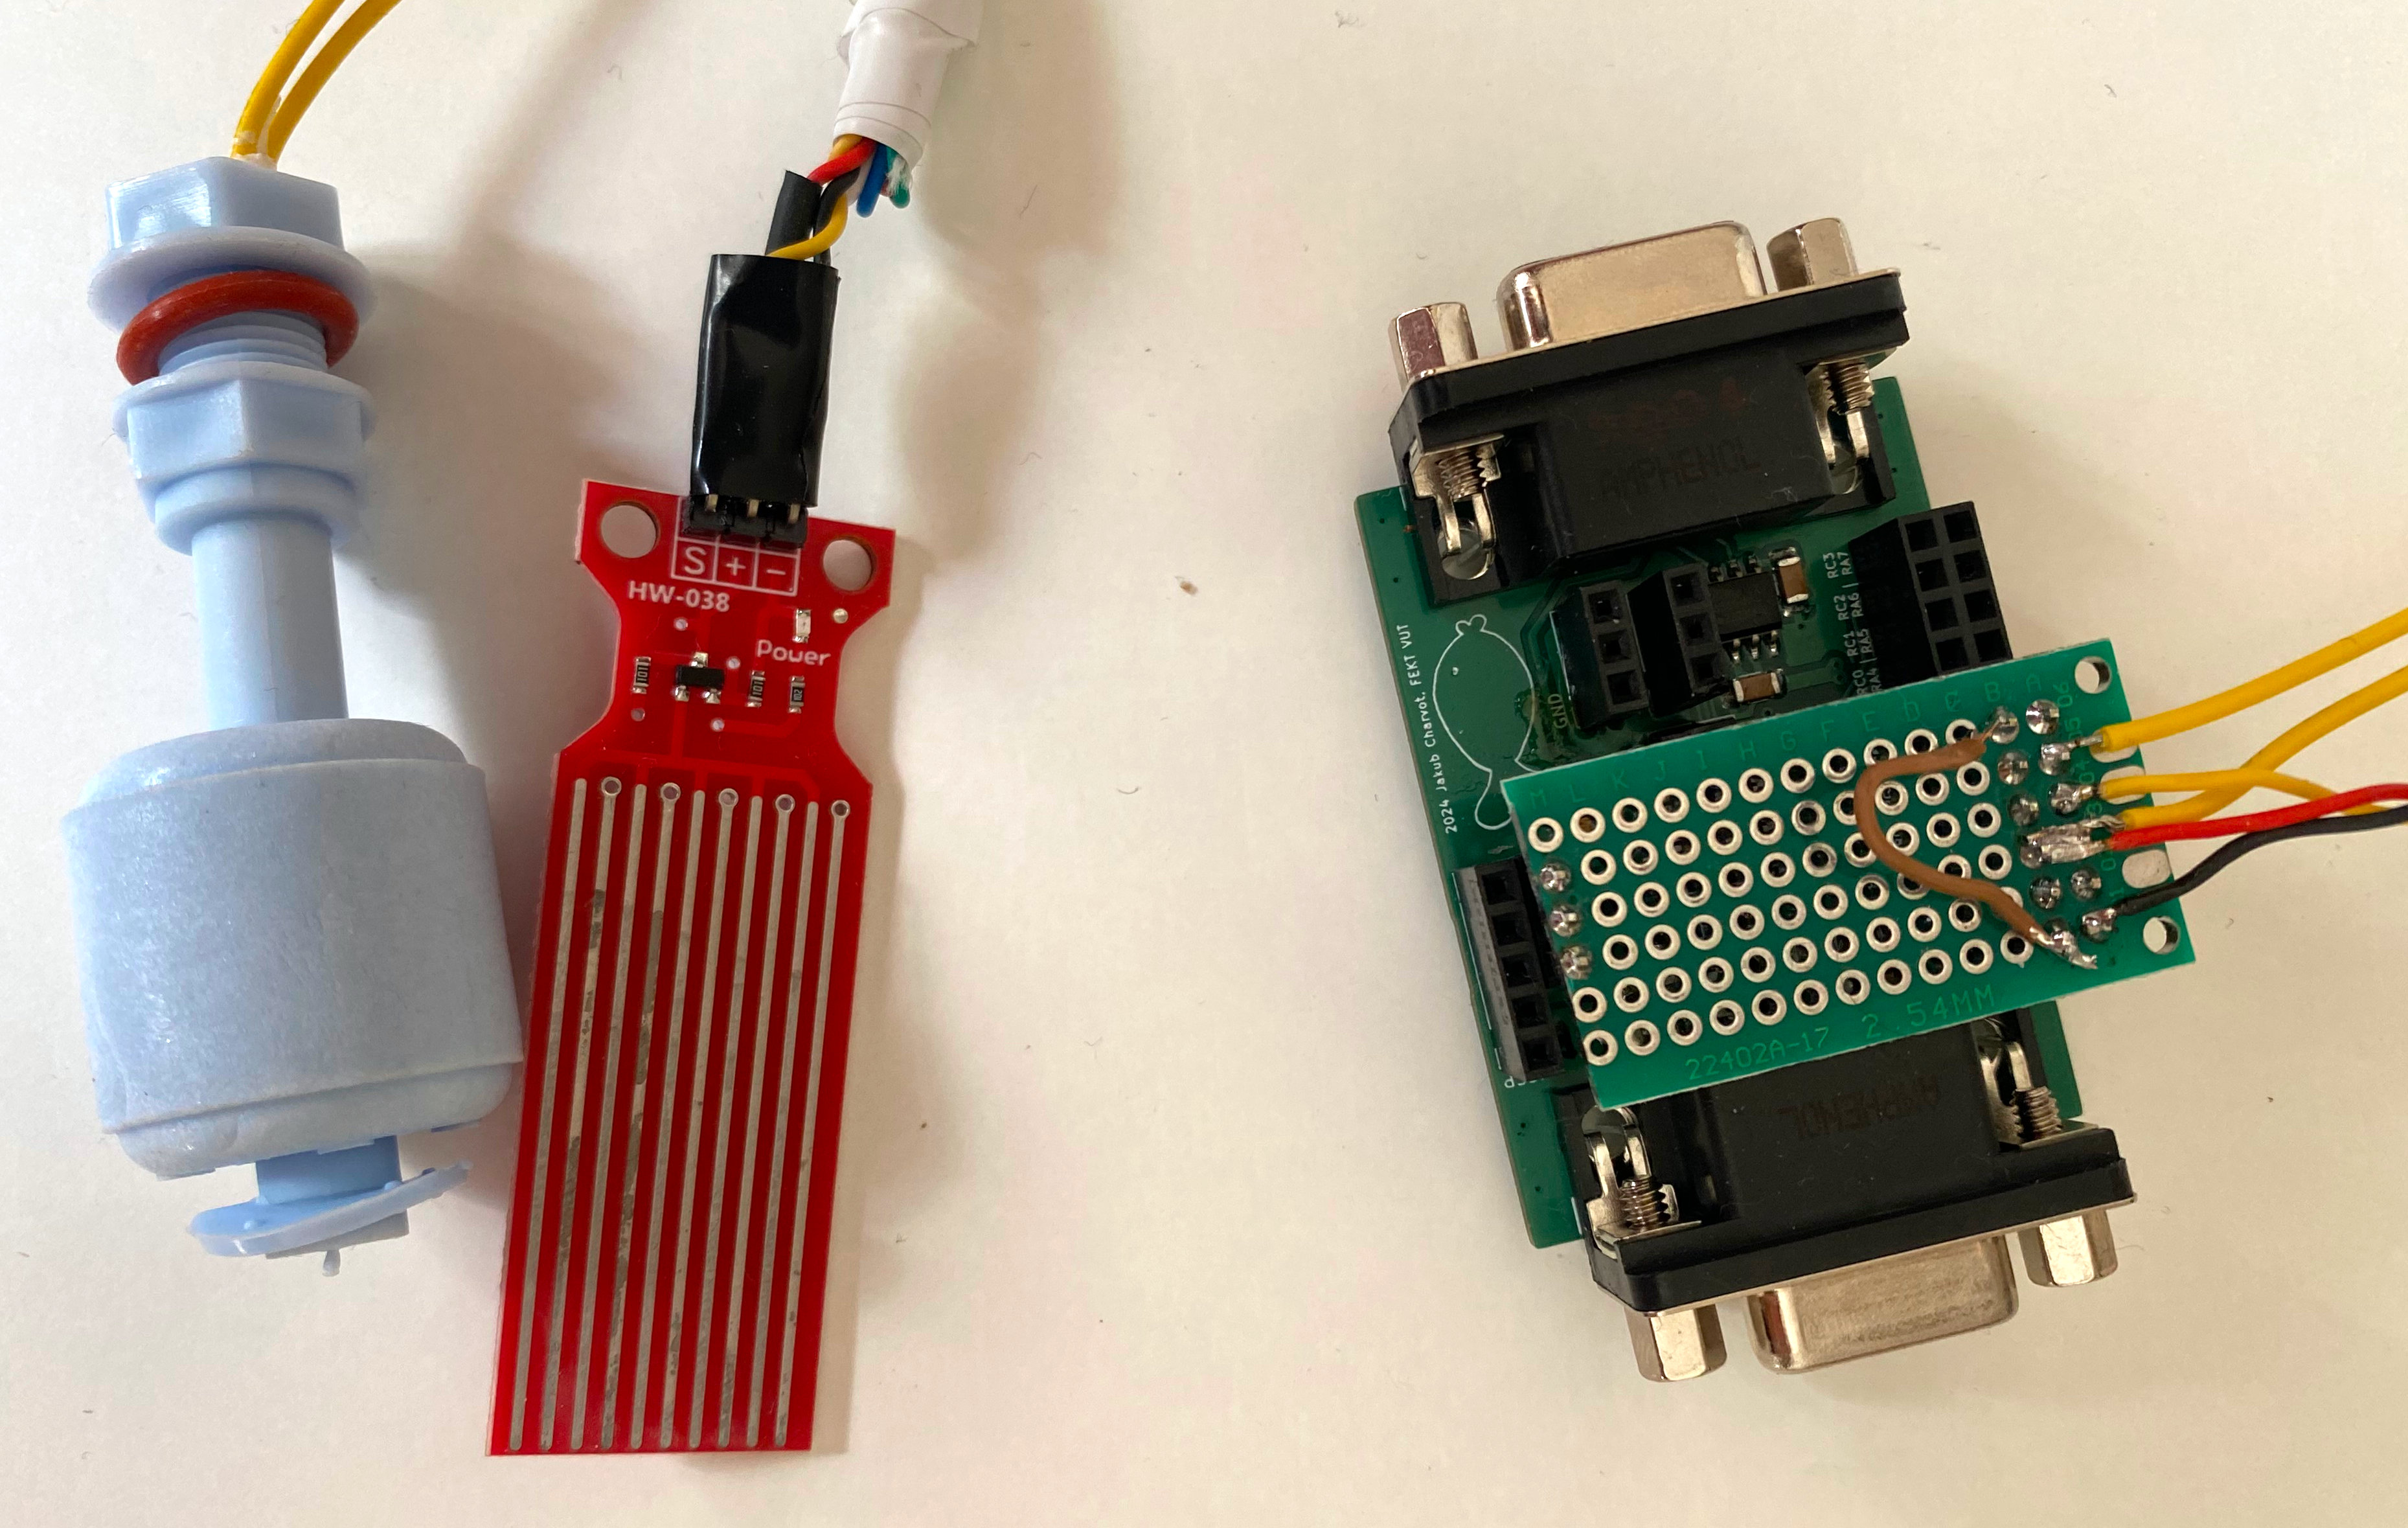
\includegraphics[width=0.8\textwidth]{obrazky/foto/sensor_hladiny.jpeg}
        \caption{Realizovaný sensor výšky hladiny.}
        \label{fig:obrazky-foto-sensor_hladiny-jpeg}
    \end{figure}
    

    K realizaci tohoto modulu jsou použity dva jednoduché sensory.Každý funguje na jiném principu a má tedy také odlišné přednosti a nedostatky, v kombinaci tak zvyšují celkovou spolehlivost modulu. Oba sensory se nachází na obr.~\ref{fig:obrazky-foto-sensor_hladiny-jpeg}, který zároveň zobrazuje realizaci jejich připojení k obecnému modulu periferií za pomocí prototypové desky. 

    \subsection{Popis zvolených sensorů}
    První ze sensorů využívá k určení výšky hladiny vodivost (potažmo odpor) vody. Obsahuje dva sety vodivých plošek, které nejsou vodivě spojeny. Při ponoření měřící části do vody začne mezi ploškami procházet slabý proud, který je přibližně úměrný velikosti ponořené části. Tento proud otevírá tranzistor, na jehož výstupu pak vzniká stejnosměrné napětí v rozsahu přiloženého napájení (zde 0 až \qty{3.3}{V}). Tento signál je přiveden na pin mikrokontroléru a následně zpracován vestaveným převodníkem. PIC18F26 obsahuje integrovanou periferii \acs{adc} s rozlišením 12 bitů, teoreticky lze tedy rozlišit \num{4296} úrovní~\cite{PIC18F26Q83}. Pro převod měřené hodnoty na výšku hladiny je potřeba sensor nejprve nakalibrovat. Byla tedy změřena přibližná výstupní hodnota pro minimální a maximální měřitelné ponoření sensoru a údaj je následně mikroprocesorem převeden na procenta. Údaj v procentech ponořené části je pro uživatele univerzálním ukazatelem nezávislým na umístění sensoru. Pro měření absolutní výšky hladiny by musel uživatel v systému nastavit výšku umístění sensoru a také ji pokaždé měnit v případě změny jeho pozice.

    Druhým sensorem je jednoduchý plovák obsahující mechanický spínač, který je při ponoření do vody rozepnut. V případě poklesu hladiny pod zvolenou úroveň je pak spínač opět sepnut.

    Propojení mikrokontroléru s oběma sensory se nachází na obr.~\ref{fig:wl-sensor-pripojeni}.

    \begin{figure}[!ht]
        \centering
        \begin{circuitikz}
            \ctikzset{resistor = european}
            % Draw the plovak sensor
            \draw (0,0) node[anchor=south,rectangle, draw, minimum width=2cm, minimum height=3cm] (plovak) {};
            \node[anchor=north] at (plovak.south) {Plovák};
            
            % Draw the pins on the plovak
            % \draw (plovak.north east) ++(0,-0.5) coordinate (pin1);
            \draw (plovak.north east) ++(0,-1.0) coordinate (pin2);
            \draw (plovak.north east) ++(0,-2) coordinate (pin3);
            % \node[left] at (pin1) {VDD};
            \node[left] at (pin2) {};
            \node[left] at (pin3) {};
            \draw (pin3) -- ++(-0.5,0) to[spst] ++(0,1) -- (pin2);
            
            % Draw the \acs{mcu}
            \draw (5,0) node[anchor=south,rectangle, draw, minimum width=4cm, minimum height=5cm] (mcu) {};
            \node[anchor=north] at (mcu.south) {PIC18F26};
            
            % Draw the pins on the \acs{mcu}
            \draw (mcu.north west) ++(0,-0.5) coordinate (mcupin1);
            \draw (mcu.north west) ++(0,-3.0) coordinate (mcupin2);
            \draw (mcu.north west) ++(0,-4)   coordinate (mcupin3);
            \draw (mcu.north east) ++(0,-2)   coordinate (mcupin4);
            \draw (mcu.north east) ++(0,-3.0) coordinate (mcupin5);
            \draw (mcu.north east) ++(0,-4)   coordinate (mcupin6);
            \node[right] at (mcupin1) {VDD};
            \node[right] at (mcupin2) {RA1};
            \node[right] at (mcupin3) {GND};
            \node[left] at  (mcupin4) {VDD};
            \node[left] at  (mcupin5) {RA0};
            \node[left] at  (mcupin6) {GND};

            % Draw the Rezistivity sensor
            \draw (10,0) node[anchor=south,rectangle, draw, minimum width=2cm, minimum height=5cm] (rsens) {};
            \node[anchor=north] at (rsens.south) {PIC18F26};
            
            % Draw the pins on the rsens
            \draw (rsens.north west) ++(0,-2) coordinate (rsenspin1);
            \draw (rsens.north west) ++(0,-3.0) coordinate (rsenspin2);
            \draw (rsens.north west) ++(0,-4) coordinate   (rsenspin3);
            \node[right] at (rsenspin1) {VDD};
            \node[right] at (rsenspin2) {SENS};
            \node[right] at (rsenspin3) {GND};
            
            % Connect plovak to \acs{mcu}
            \draw (mcupin1) -- ++(-1,0);
            \draw (pin2) -- (mcupin2);
            \draw (pin3) -- (mcupin3);

            % Connect rsens to \acs{mcu}
            \draw (rsenspin1) -- (mcupin4);
            \draw (rsenspin2) -- (mcupin5);
            \draw (rsenspin3) -- (mcupin6);

            % Add pull-up resistor
            \draw (mcupin1) ++(-1,0) to[R, l_=100k, -*] ++(0,-2.5);
        
        \end{circuitikz}
        \caption{Připojení sensorů hladiny k \acs{mcu}.}
        \label{fig:wl-sensor-pripojeni}
    \end{figure}